\documentclass[10pt,twocolumn]{article}
\usepackage{times}
\usepackage[margin=0.75in,top=1in]{geometry}
\usepackage{graphicx}
\usepackage{booktabs}
\usepackage{amsmath}
\usepackage{amssymb}
\usepackage{hyperref}
\usepackage{microtype}
\usepackage{xcolor}
\usepackage{caption}
\usepackage{subcaption}
\usepackage{enumitem}
\usepackage{multirow}

\setlength{\columnsep}{0.25in}

\title{\textbf{Right to Be Forgotten in LLMs: A Cross-Platform Empirical Audit of Erasure Control Failures}}

\author{
  Taiwo Olabamipe \\
  University of Central Florida \\
  \texttt{tal17847@ucf.edu}
  \and
  Xueqiang Wang \\
  University of Central Florida \\
  \texttt{xueqiang.wang@ucf.edu}
  \and
  Yao Li   \\
  University of Central Florida \\
  \texttt{yao.li@ucf.edu}
}

\date{}

\begin{document}

\maketitle

% ----------------------------------------------------------------
\begin{abstract}
\textit{
This study presents }
\end{abstract}
% ----------------------------------------------------------------

\section{Introduction}

The right to erasure, enshrined in Article 17 of the General Data

This study addresses the following research questions, split by system and
user side, plus their divergence:

\begin{itemize}[leftmargin=*]
  \item[] \textbf{RQ1} (system, behavior): How do commercial LLM chatbots
    actually handle data erasure requests?
  \item[] \textbf{RQ2} (system, policy gap): Where does observed erasure
    behavior contradict each platform's stated policy?
  \item[] \textbf{RQ3} (user, expectation \& verification): What do users
    believe deletion accomplishes, and do they verify that it worked?
  \item[] \textbf{RQ4} (user, sensitivity): Does data sensitivity change
    deletion method choice, willingness to delete, or expected effort/loss?
  \item[] \textbf{RQ5} (divergence): Where does user expectation diverge
    most from audited platform behavior, and who bears that gap?
\end{itemize}

The participatory survey reported in this paper addresses RQ3 and RQ4; RQ1,
RQ2, and RQ5 require the companion technical audit across six commercial
platforms, reported separately.

\section{Background and Related Work}

\section{Participatory Study}

\subsection{What Users Know About Memory and Deletion}

Of 219 raw responses, 1 was dropped for failing the attention check and 36
were excluded for never having deleted data from an AI chatbot before,
leaving 182 eligible participants and a paired analysis base of $n=177$ who
completed both the less-sensitive and more-sensitive scenario blocks.

\textbf{The sample skews young, educated, and experienced with AI chatbots.}
Table~\ref{tab:demographics} summarizes demographics: 73\% of participants
are under 45, the majority identify as male (58.8\%), and 62.1\% hold a
bachelor's degree or higher. All participants were US-based with prior
chatbot experience, per the study's eligibility criteria. As shown in
Figure~\ref{fig:ai-tenure}, ChatGPT (99.4\%) and Gemini (92.7\%) are
near-universal among participants, Claude and Copilot are each used by
two-thirds (67.8\%), and Perplexity and Deepseek are both the least-used and
most recently adopted platforms.

\textbf{Participants show strong baseline privacy knowledge, with one
consistent blind spot.} On a 6-item objective knowledge check spanning the
right to be forgotten, chatbot memory, and training data, participants
averaged 5.06/6 correct (median 5.0/6; Table~\ref{tab:demographics}), and
46.3\% answered all six items correctly. The weakest item was whether
chatbots access only public user data (70.1\% correct; 29.9\% incorrectly
believe they do). The strongest was recognizing that conversations may be
used to train future models (93.8\% correct).

\begin{table}[t]
\centering
\caption{Sample Demographics ($n=177$). Skews young (73\% under 45),
majority male (58.8\%), and highly educated (62.1\% bachelor's degree or
higher). Participants also show high baseline privacy knowledge
(mean 5.06/6, median 5.0/6).}
\label{tab:demographics}
\small
\setlength{\tabcolsep}{3.5pt}
\begin{tabular}{llcc}
\toprule
Variable & Response & $n$ & \% \\
\midrule
\multirow{6}{*}{Age}
 & 25--34 & 56 & 31.6 \\
 & 35--44 & 45 & 25.4 \\
 & 18--24 & 29 & 16.4 \\
 & 45--54 & 27 & 15.3 \\
 & 55--64 & 17 & 9.6 \\
 & 65+    & 3  & 1.7 \\
\midrule
\multirow{3}{*}{Gender}
 & Man               & 104 & 58.8 \\
 & Woman             & 72  & 40.7 \\
 & Prefer not to say & 1   & 0.6 \\
\midrule
\multirow{6}{*}{Education}
 & Bachelor's degree      & 75 & 42.4 \\
 & Graduate/professional  & 35 & 19.8 \\
 & Some college, no degree & 30 & 16.9 \\
 & Associate's/technical  & 19 & 10.7 \\
 & High school/GED        & 15 & 8.5 \\
 & Some high school or less & 3 & 1.7 \\
\midrule
Privacy Knowledge (0--6) & $M=5.06$, $Mdn=5.0$ & --- & --- \\
\bottomrule
\end{tabular}
\end{table}

\begin{figure}[t]
\centering
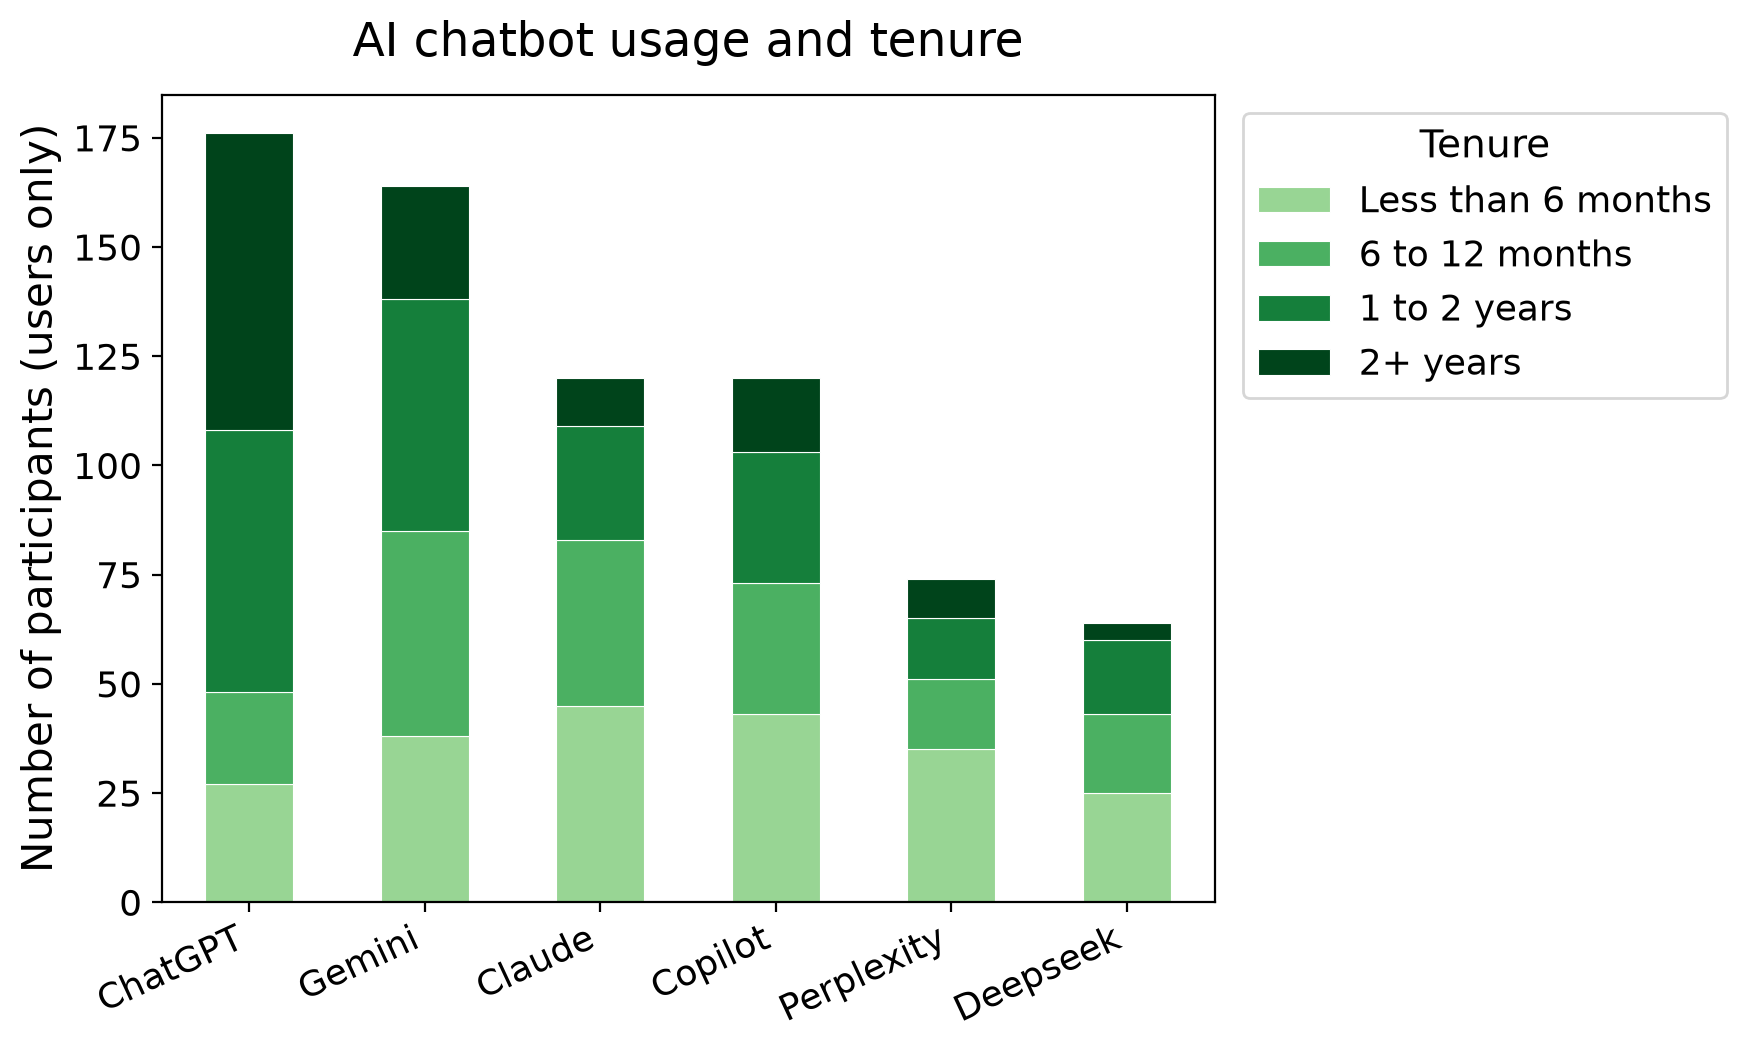
\includegraphics[width=\linewidth]{figures/fig1_ai_tenure.png}
\caption{AI chatbot usage and tenure ($n=177$). ChatGPT and Gemini are
near-universal; Perplexity and Deepseek are least used and most recently
adopted.}
\label{fig:ai-tenure}
\end{figure}

\subsection{Deletion Expectations and the Sensitivity Effect}

\textbf{``Delete this single conversation'' dominates method selection in
both scenarios, but the shift with sensitivity is not statistically
significant.} As shown in Figure~\ref{fig:method-selection}, it accounts for
84/177 (47.5\%) of choices in the less-sensitive scenario and 80/177 (45.2\%)
in the more-sensitive one -- roughly three times the next most common method,
``Clear all conversation history'' (33 and 40, respectively). Only four of
the seven offered methods clear the $n\geq14$ reporting floor used for
inferential testing in every scope; the remaining three (Clear all saved
memories, Privacy dashboard, Delete my account) are reported descriptively
only. The overall distribution shift across all seven methods is not
statistically significant (Stuart-Maxwell, $p=.393$).

\begin{figure}[t]
\centering
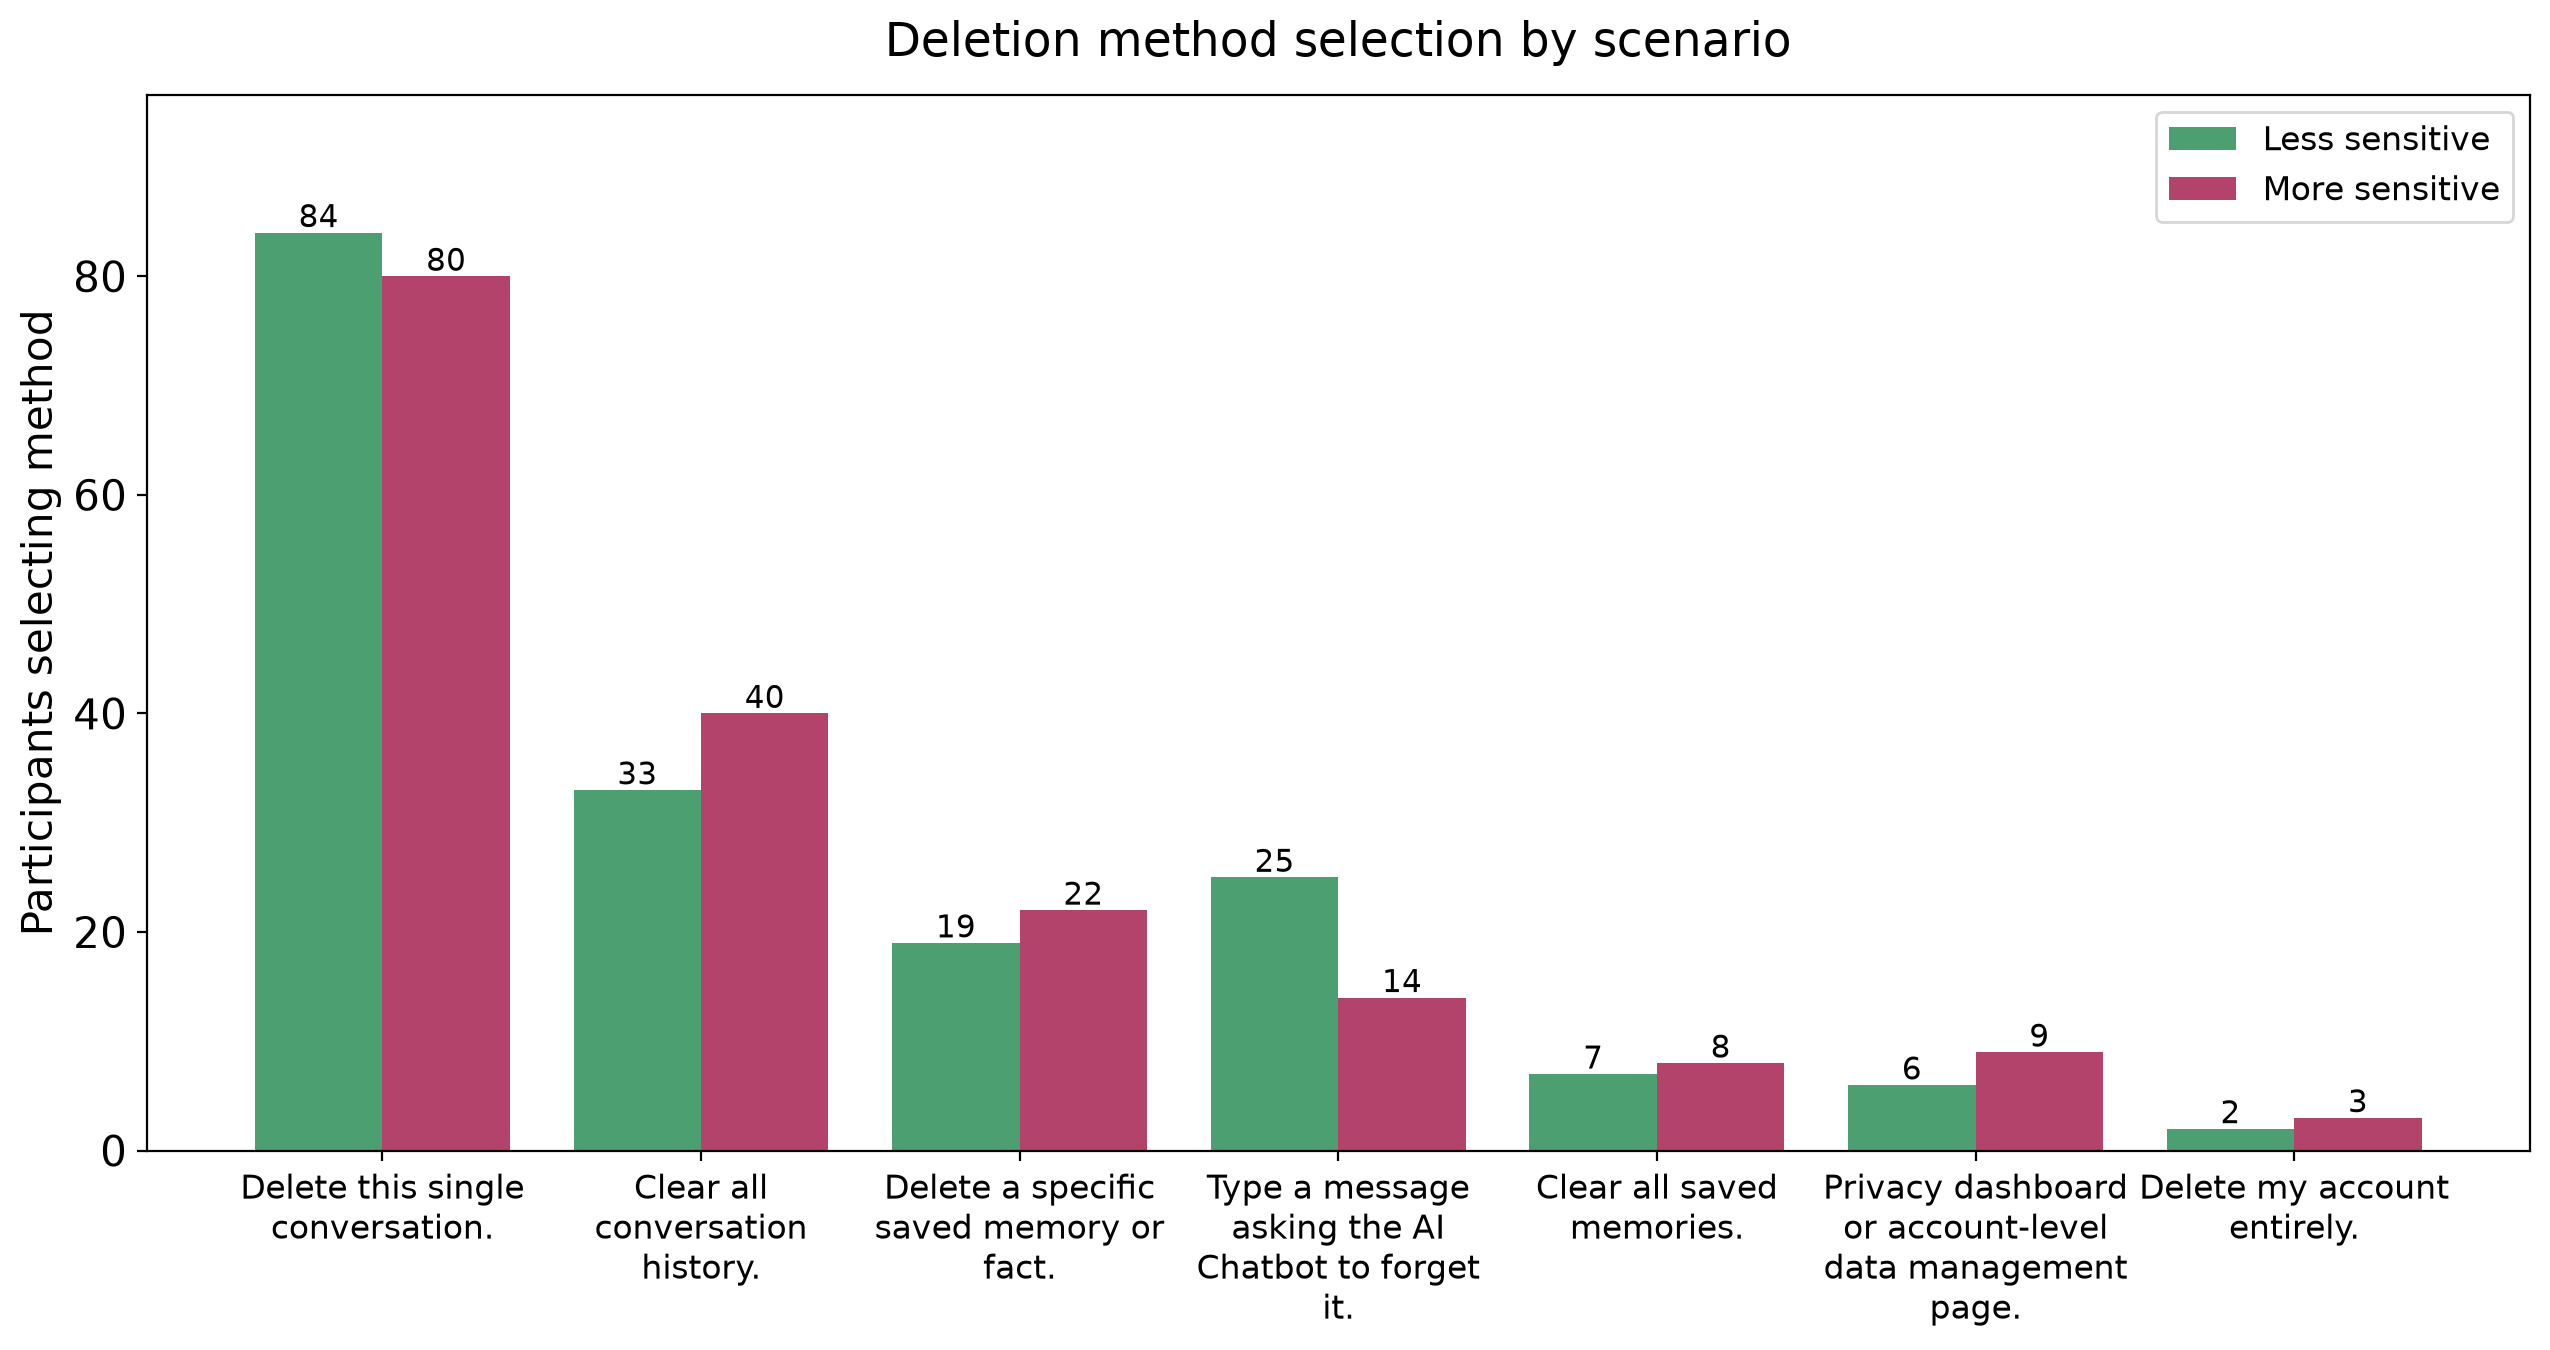
\includegraphics[width=\linewidth]{figures/fig2_method_selection.png}
\caption{Deletion method selection by scenario ($n=177$, paired). ``Delete
this single conversation'' dominates in both scenarios; the overall
distribution shift is not statistically significant (Stuart-Maxwell,
$p=.393$).}
\label{fig:method-selection}
\end{figure}

\textbf{Methods separate clearly on effort, but barely on protection or
benefit loss.} ``Delete a specific saved memory or fact'' is rated
highest-effort and highest-benefit-loss in every scope (pooled $M=2.45$
effort, $M=3.43$ benefit loss), while ``Delete this single conversation'' is
rated lowest-effort throughout (pooled $M=1.68$). Protection ratings are far
more compressed across methods (pooled range 3.65--3.80); see
Figure~\ref{fig:crowning-combined} below for the median-based, significance-
annotated version of this comparison.

\textbf{No deletion method is ever the single statistically best choice on
any scale.} Kruskal-Wallis tests find no significant difference between
methods on protection or benefit loss, in any scope -- pooled, less-, or
more-sensitive (all $p>.15$, 6/6 tests null). Effort is the only scale with
a significant omnibus difference in every scope (pooled $H=19.54$, $p<.001$;
less $H=18.42$, $p<.001$; more $H=16.98$, $p<.001$; Figure~\ref{fig:crowning-combined}),
but even there no method clears every pairwise post-hoc comparison.
``Delete this single conversation'' has the best (lowest) effort point
estimate in the pooled and less-sensitive scopes and significantly
outperforms ``Delete a specific saved memory or fact'' ($p<.001$ both), but
is statistically indistinguishable from ``Clear all conversation history''
and ``Type a message asking the AI Chatbot to forget it.'' In the
more-sensitive scope the ranking flips -- ``Type a message...'' has the
lowest raw mean -- but it does not significantly beat any other method
there. The data support a narrow claim only: ``Delete this single
conversation'' is reliably lower-effort than ``Delete a specific saved
memory,'' not that it is the single lowest-effort method overall.

\begin{figure}[t]
\centering
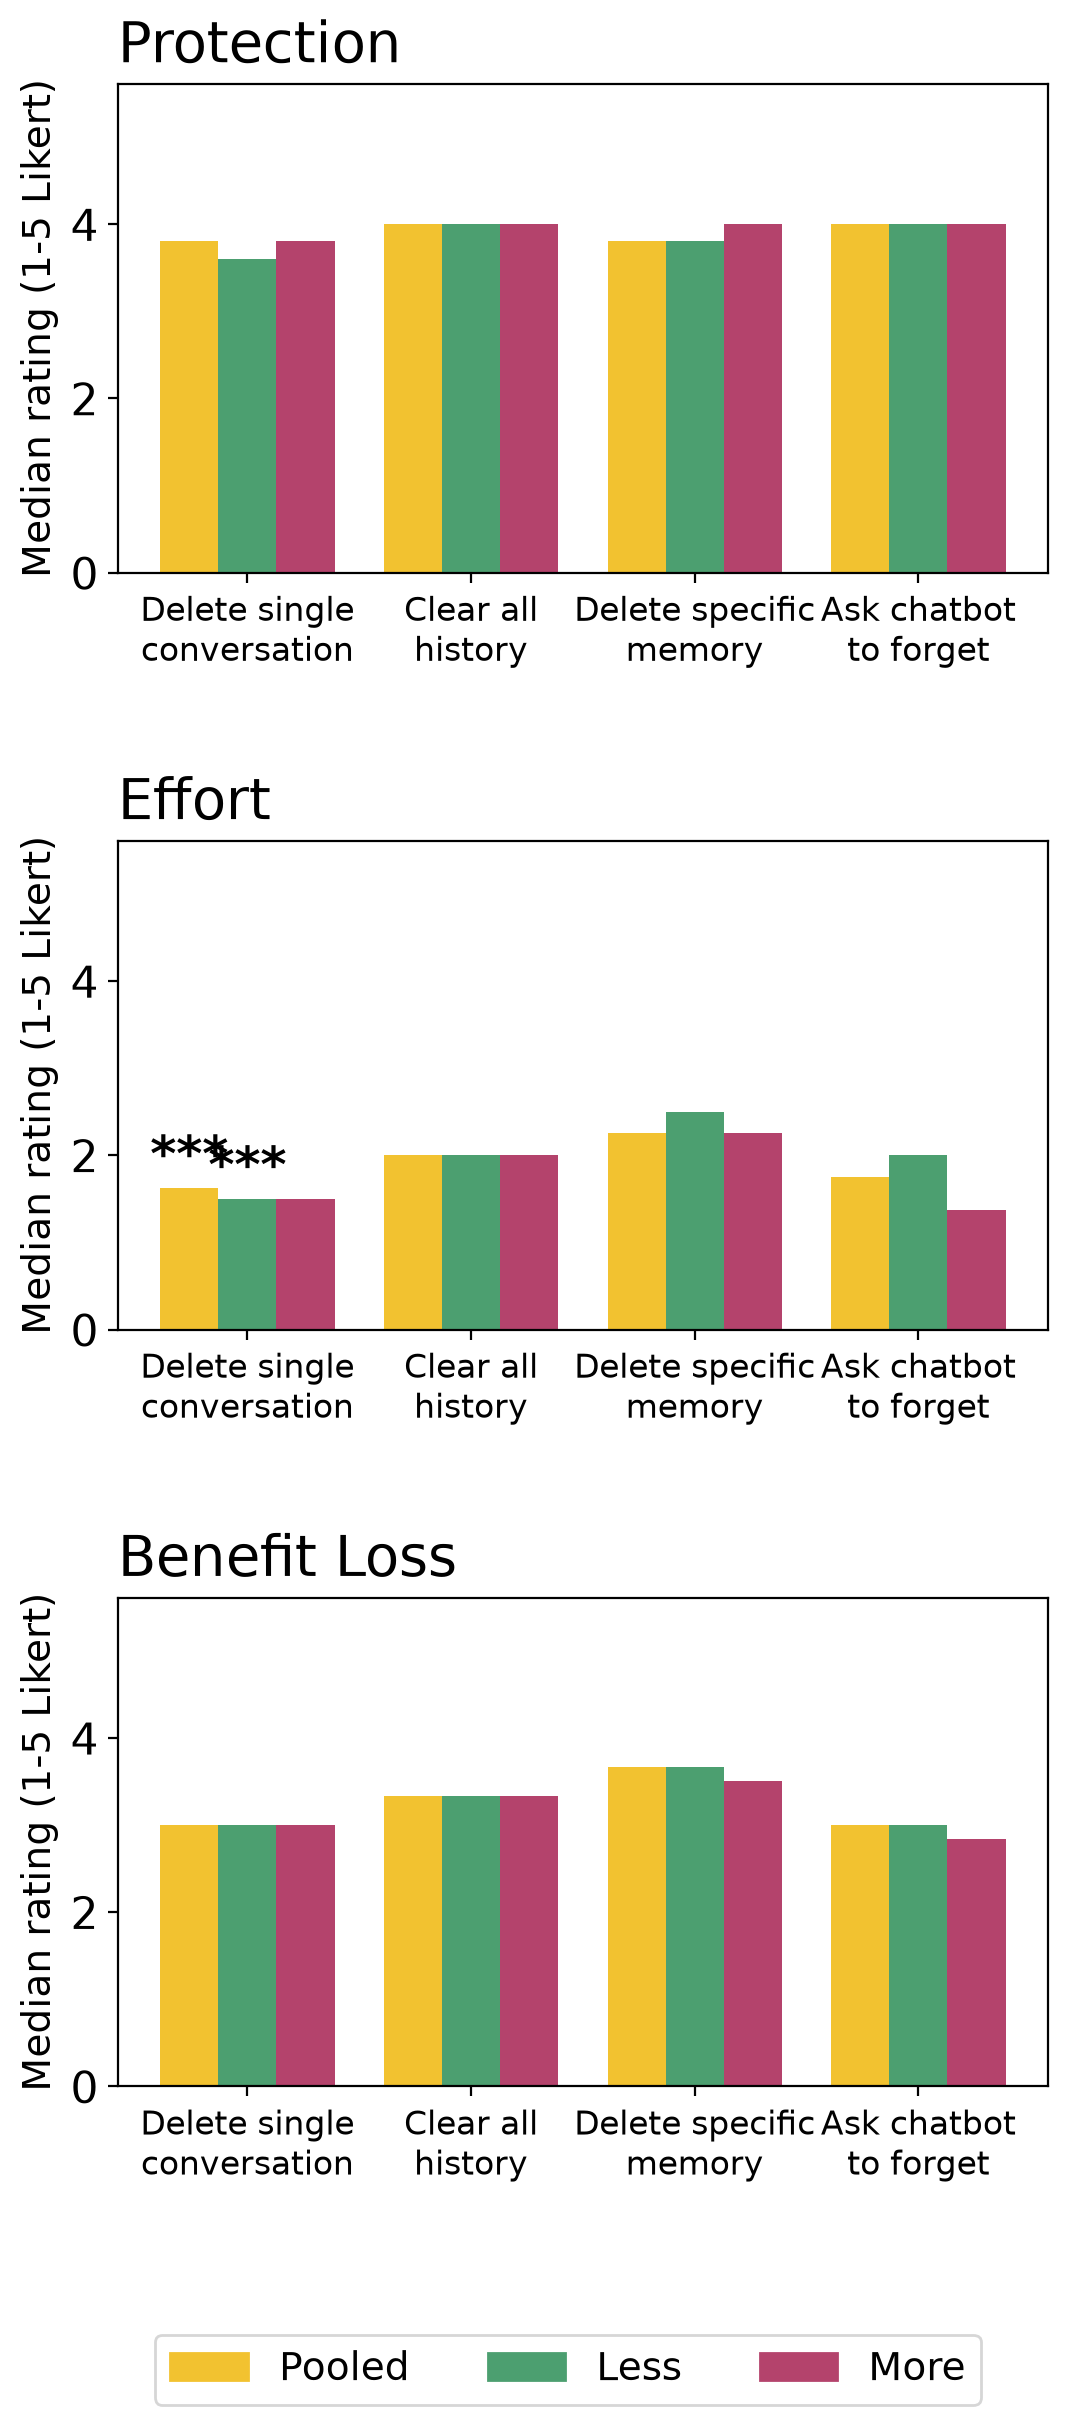
\includegraphics[width=\linewidth]{figures/fig_crowning_combined.png}
\caption{Median protection, effort, and benefit-loss ratings by deletion
method (pooled / less-sensitive / more-sensitive). No method is significantly
best on any scale, except: ``Delete this single conversation'' is
significantly lower-effort than ``Delete a specific saved memory'' in the
pooled and less-sensitive scopes ($p<.001$).}
\label{fig:crowning-combined}
\end{figure}

\textbf{Willingness to delete and perceived protection both rise
significantly as data sensitivity increases; effort and perceived loss do
not.} This is a different question from method choice above -- it asks
whether sensitivity itself, independent of which method someone uses, moves
these ratings. Paired comparison of the same $n=177$ participants across the
less- and more-sensitive scenarios (Wilcoxon signed-rank) shows willingness
to delete rising from $M=3.98$ to $M=4.37$ ($+0.39$, $p<.001$, $r=.55$, the
largest effect in this study) and perceived protection rising from $M=3.66$
to $M=3.79$ ($+0.13$, $p<.001$, $r=.38$). Effort ($+0.03$) and benefit loss
($+0.04$) show no significant change (both ns). Protection is the notable
case: \emph{which method} someone uses has no effect on perceived
protection in any scope (above), yet \emph{how sensitive the data feels}
moves it significantly -- two independent findings about protection, not a
contradiction. Benefit loss is the one scale unmoved on either axis.

\textbf{Method switching is common overall, and one method shows a
significant decline under higher sensitivity.} 64\% of participants
(113/176) select the same deletion method in both scenarios, while 36\%
(63/176) switch. The aggregate 7-category distribution does not shift
significantly (Stuart-Maxwell, stat$=6.28$, $df=6$, $p=.393$). Ranked by
raw net change (added minus dropped), ``Clear all conversation history''
gains the most adopters ($+7$) as sensitivity rises, while ``Type a message
asking the AI Chatbot to forget it'' loses the most ($-11$; 15 dropped vs.\
4 added, $p=.019$) -- participants become significantly less likely to rely
on a conversational request when the data feels more sensitive. Every other
individual method's shift is non-significant. Individual-level churn is
real -- over a third of participants change their answer -- but only this
one method shows a clean, significant directional pattern.

\textbf{Beliefs about what deletion does and how people verify it form a
genuine hierarchy within each scenario, dominated by a training-data blind
spot.} Cochran's Q confirms both rankings are far from a flat distribution
(expectation: $Q=245.25$, $p<.001$; verification: $Q=142.99$, $p<.001$,
less-sensitive scenario; both replicate in the more-sensitive scenario).
``Permanently deleted'' is the most commonly held belief (55.4\% less,
62.4\% more), while ``not used for training'' is the least- or near-least-
endorsed belief for every reportable method in both scenarios (15--37\%) --
roughly two-thirds to five-sixths of participants do not expect deletion to
stop their data from training the model, regardless of which method they
use. On verification, ``did NOT know how to check'' is the single most
common response in both scenarios ($\approx$45\%), well ahead of any active
verification behavior (Figure~\ref{fig:expectation-verification}).

\begin{figure}[t]
\centering
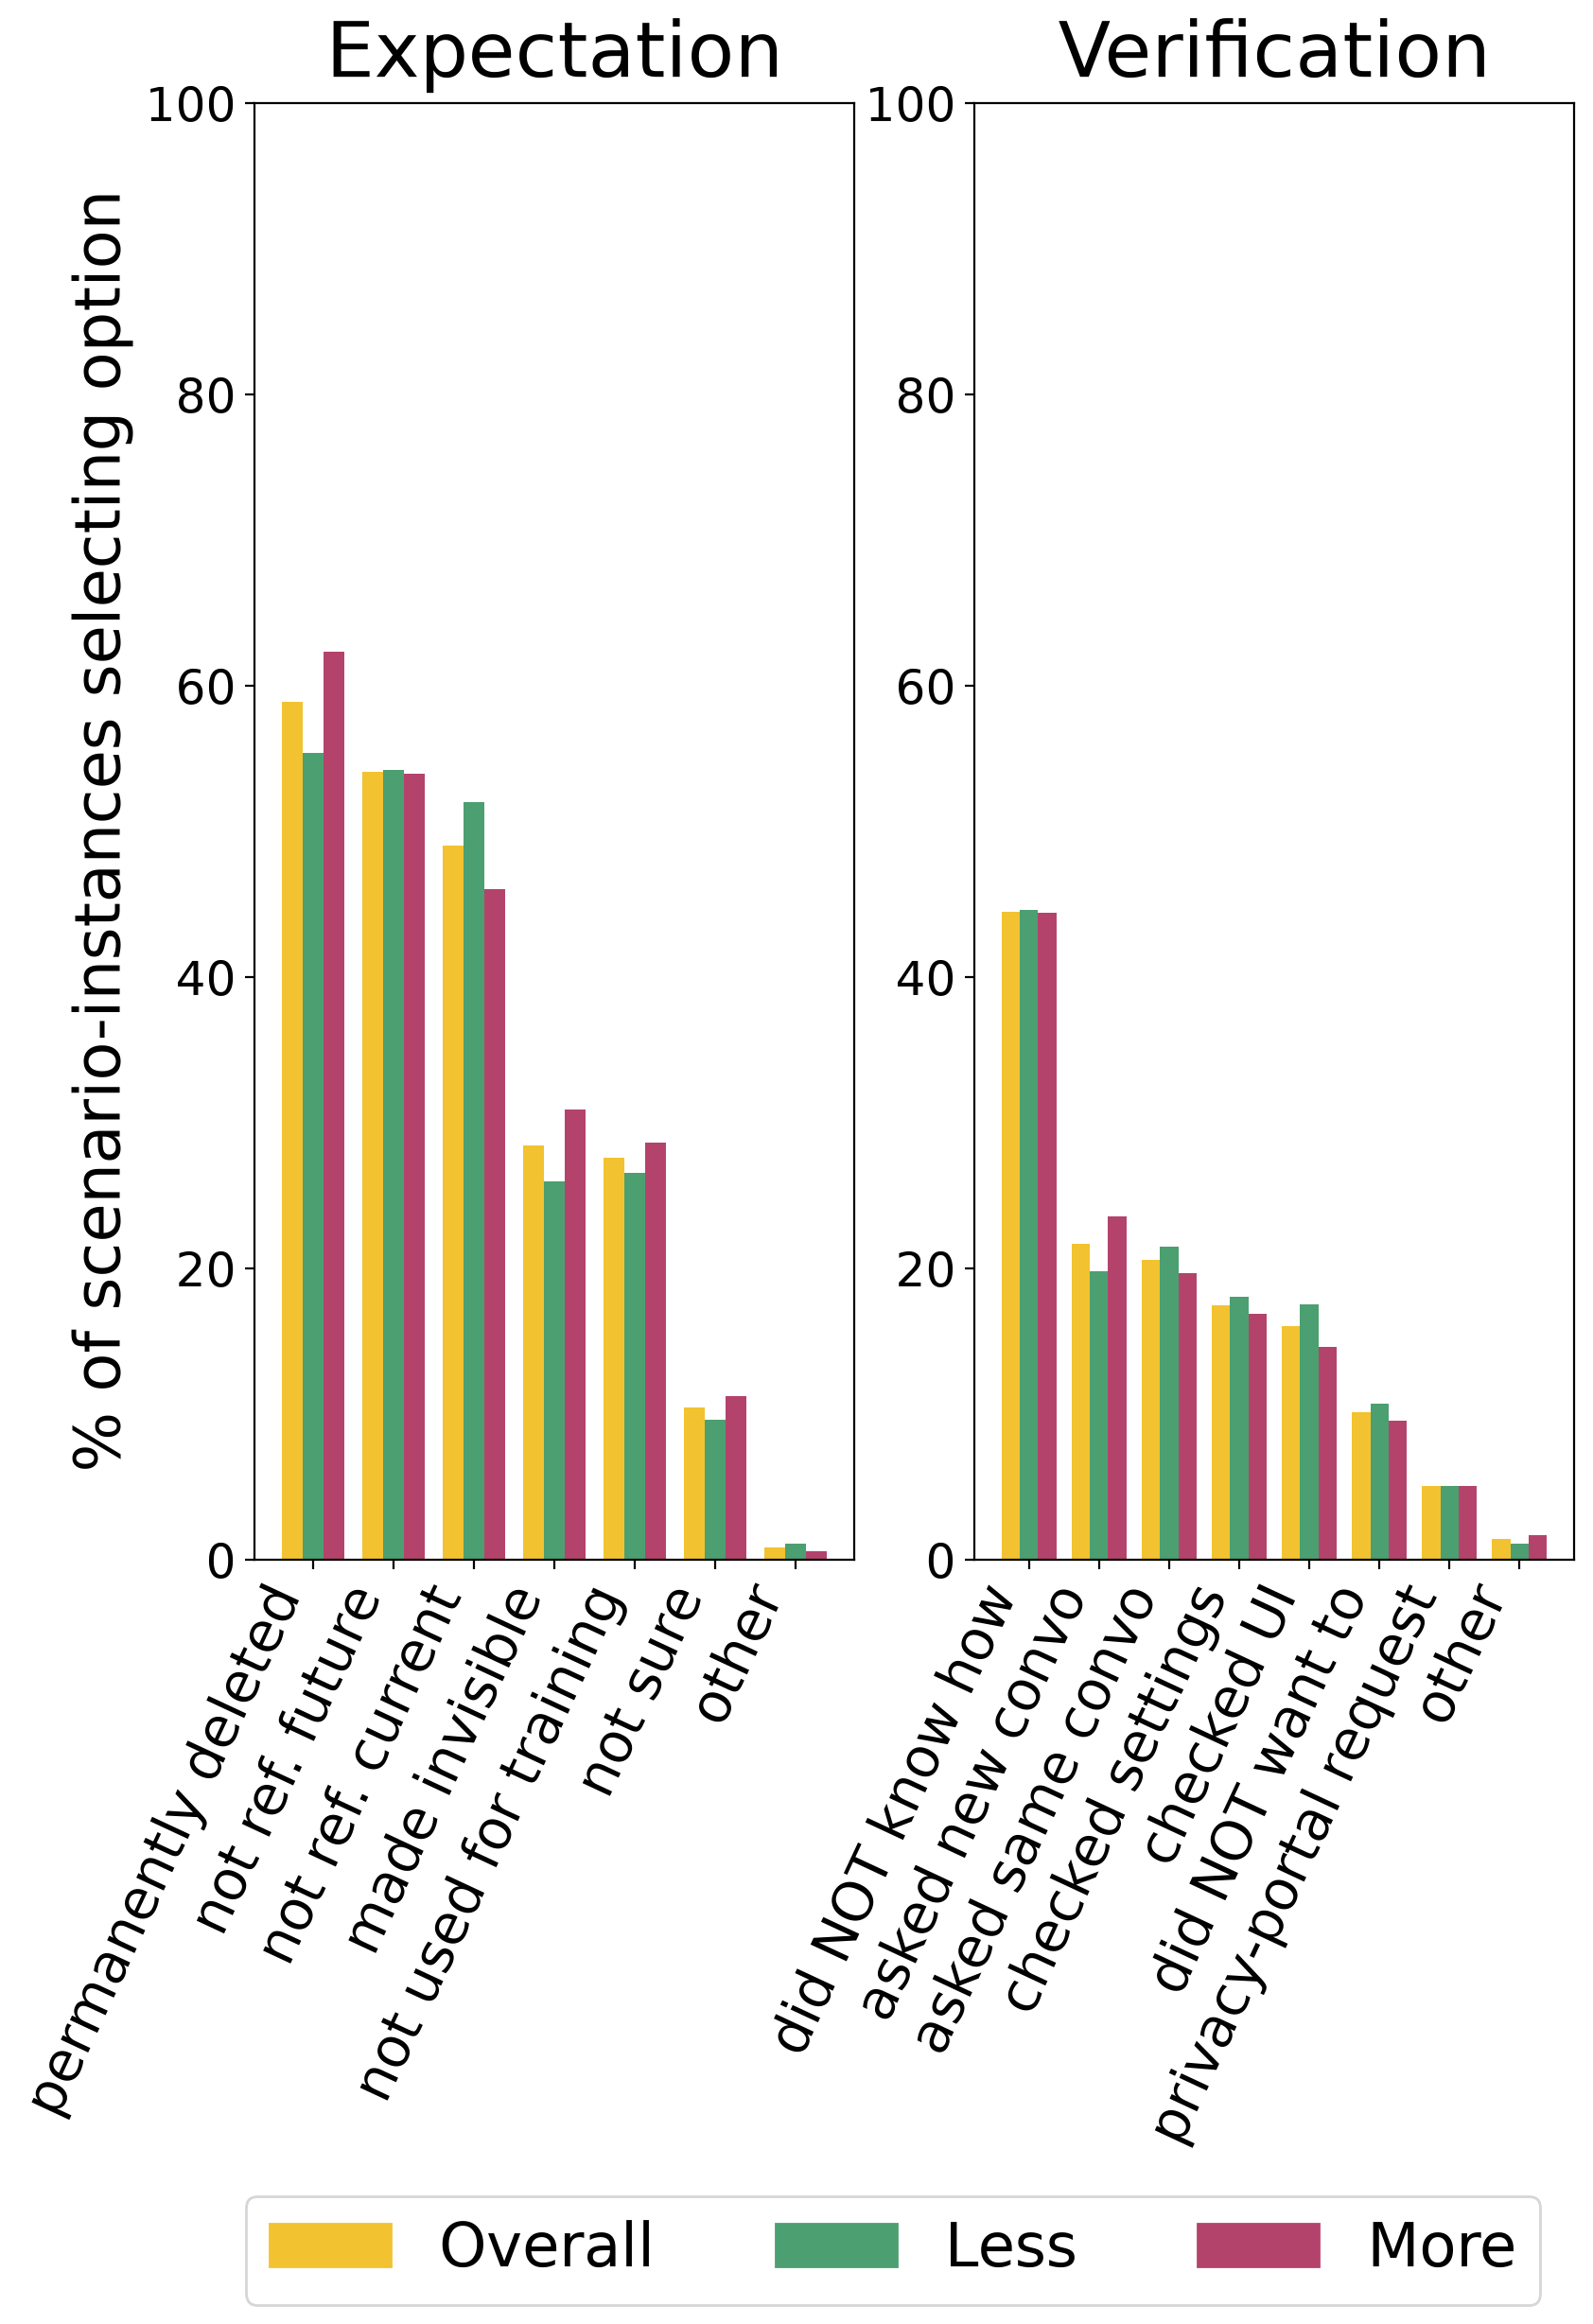
\includegraphics[width=\linewidth]{figures/fig_expectation_verification.png}
\caption{Expectation and verification option selection rates (overall /
less-sensitive / more-sensitive). ``Permanently deleted'' is the most common
belief about what deletion does; ``did NOT know how to check'' is the most
common verification response, in every scope.}
\label{fig:expectation-verification}
\end{figure}

\textbf{Deletion method has no significant association with stated
expectation, pooled across both scenarios.} Table~\ref{tab:contingency}
breaks down the same four qualifying methods against the top expectation
options, as \% of each method's own $n$ (comparable across methods; raw
counts scale with method popularity and are not). Testing all seven
expectation options against method choice (chi-square where all expected
counts $\geq5$, Fisher's exact otherwise, Holm-corrected within the family
of seven), none survive correction -- closest is ``made invisible/hidden''
($p_{raw}=.049$, $p_{holm}=.344$) -- and effect sizes are uniformly small
(Cram\'er's $V\leq.19$). Which method someone picks predicts nothing
statistically about what they expect it to do, matching the per-scenario
tests below.

\begin{table}[t]
\centering
\caption{Deletion Method $\times$ Expectation (Pooled, Deduped per
Respondent), \% of Each Method's Own $n$}
\label{tab:contingency}
\small
\setlength{\tabcolsep}{3pt}
\begin{tabular}{lcccc}
\toprule
Method ($n$) & Perm. & Not ref. & Not ref. & No longer \\
 & deleted & (current) & (future) & trained \\
\midrule
Single conv. (105)  & 59.0 & 43.8 & 51.0 & 27.6 \\
Clear history (50)  & 54.0 & 41.0 & 45.0 & 21.0 \\
Specific memory (30) & 65.0 & 63.3 & 58.3 & 16.7 \\
``Forget'' msg (29) & 56.9 & 56.9 & 53.4 & 32.8 \\
\bottomrule
\end{tabular}
\vspace{4pt}

\footnotesize{\textbf{Concise conclusion:} no significant association
between deletion method and expectation (all $p_{holm}\geq.344$; Cram\'er's
$V\leq.19$ throughout) -- method choice does not predict what a user expects
deletion to accomplish. Columns shown are the three dominant expectations
(top-3 for every method) plus the training-data blind spot; ``made
invisible/hidden'' and ``not sure/other'' omitted for space, included in the
significance test above.}
\end{table}

\textbf{Verification behavior differs significantly by method; beliefs
about what deletion does mostly do not.} In the less-sensitive scenario,
three verification behaviors vary significantly by method: ``asked in same
conversation'' ($p<.001$), ``asked in new conversation'' ($p=.002$), and
``did NOT know how to check'' ($p=.001$). The same three verification
behaviors, with ``checked settings'' replacing ``asked in new
conversation,'' vary significantly by method in the more-sensitive scenario
(``asked in same conversation'' $p=.005$, ``checked settings'' $p=.006$,
``did NOT know how to check'' $p=.044$). Expectations are far more stable
across methods: no expectation option varies significantly by method in the
less-sensitive scenario, though two do in the more-sensitive one --
``not referenced in current conversation'' ($p=.008$) and ``not referenced
in future conversation'' ($p=.030$). This mirrors the earlier effort
finding: the easiest methods to invoke (lowest effort, Figure~\ref{fig:crowning-combined}) are
also the ones users are least equipped to verify.

\textbf{Verification tracks stated confidence, but miscalibration remains
severe and does not improve when stakes rise.} An ordinal trend test
confirms that participants reporting higher confidence a deletion worked
were more likely to have verified it, in both scenarios (less: $z=2.50$,
$p=.012$; more: $z=2.23$, $p=.026$). Even so, base rates of verification
are low throughout: among participants ``not at all confident'' the
deletion worked, 81.8\% never verified in the less-sensitive scenario and
88.9\% never verified in the more-sensitive one -- if anything slightly
worse, not better, when the data is more sensitive.

\textbf{Participants consistently report an ideal method different from
the one they actually used, and this gap widens as sensitivity rises.}
Paired comparison of used-vs-ideal method selection is significant for
every method except ``Delete my account entirely'' in the less-sensitive
scenario (all $p<.001$; e.g., ``Ask chatbot to forget'': 6 used-only vs.\
64 ideal-only). In the more-sensitive scenario all seven methods reach
significance, including ``Delete my account'' ($p=.022$). The gap is
directional throughout -- far more participants nominate a method as ideal
than actually use it, never the reverse -- and widens under higher
sensitivity for the largest methods: ``Ask chatbot to forget'' grows from
32.8 to 42.1 percentage points, ``Delete a specific saved memory'' from
20.3 to 29.2. The disconnect between stated preference and actual behavior
is largest exactly when the stakes are highest.

\textbf{Neither age nor chatbot tenure moderates the rating scales in
either scenario; each predicts method choice in one scenario only.}
Kruskal-Wallis tests find no significant effect of age group or ChatGPT
tenure on protection, effort, benefit loss, or willingness to delete, in
either scenario (all $p>.14$, 16/16 tests null). Age group significantly
predicts \emph{which method} someone selects in the less-sensitive scenario
(Fisher's exact, $p=.015$, Cram\'er's $V=.229$) but not in the
more-sensitive one ($p=.080$); ChatGPT tenure shows the reverse pattern,
predicting method choice in the more-sensitive scenario ($p=.013$,
$V=.207$) but not the less-sensitive one ($p=.121$). Both associations are
modest in size ($V\approx.21$--$.23$) -- real but not large -- and neither
demographic variable moderates how protective, effortful, or costly a
method feels to use.

\textbf{Protection, effort, and benefit loss are statistically distinct
constructs, justifying their treatment as three separate outcomes above.}
Table~\ref{tab:discriminant-validity} reports pooled pairwise Spearman
correlations among the three scales. All three pairs fall well below the
$|\rho|\geq0.8$ threshold conventionally used to flag construct redundancy.
Protection is essentially uncorrelated with the other two scales
($\rho=-0.057$ with effort, $\rho=0.129$ with benefit loss, both ns).
Effort and benefit loss show the one significant relationship in the data
($\rho=0.305$, $p<.001$) -- a small-to-moderate positive association, not
redundancy: participants who rate a method as more effortful also tend to
rate it as costing them more, consistent with the pattern above where
``Delete a specific saved memory'' rates highest on both.

\begin{table}[t]
\centering
\caption{Discriminant Validity: Spearman Correlations Among Protection, Effort, and Benefit Loss (Pooled, $n=177$)}
\label{tab:discriminant-validity}
\begin{tabular}{lccc}
\toprule
 & Protection & Effort & Benefit Loss \\
\midrule
Protection   & --- & $-0.057$ & $0.129$ \\
Effort       & $-0.057$ & --- & $0.305^{***}$ \\
Benefit Loss & $0.129$ & $0.305^{***}$ & --- \\
\bottomrule
\end{tabular}
\vspace{4pt}

\footnotesize{Cell values are Spearman's $\rho$ (correlation strength) between
each pair, pooled across both scenarios. $^{*}p<.05$, $^{**}p<.01$,
$^{***}p<.001$. Only effort--benefit loss is statistically significant.}
\end{table}

\section*{Discussion}




\section*{Limitations}

\section*{Conclusion}



\end{document}
